\chapter{Inverse Trigonometric Functions}

A wheelchair ramp must be gentle: building codes allow it to rise at most
1 meter for every 12 meters it runs. What angle is that? You know
$\tan\theta = \frac{1}{12}$. To get from the ratio back to the angle, you
need to run tangent backward. That is what inverse trigonometric functions
do.

In the inverses chapter, an inverse was a machine that turns $y$ back into
$x$.\index{inverse trigonometric functions} Let us start with $\sin$ and
its inverse, $\sin^{-1}$, also called \index{arcsine}$\arcsin$. (Careful:
$\sin^{-1} x$ means the inverse function, not $\frac{1}{\sin x}$.)

\begin{center}
	\begin{figure}
	\centering
		\begin{tikzpicture}
			\begin{axis}
			[axis lines = center, 
			xlabel=$x$,
			xmin=-3.142, 
			xmax=6.283, 
			xtick={-3.142, -1.571, 0, 1.571, 3.142, 4.712, 6.283}, 
			xticklabels={$-\pi$, $\frac{-\pi}{2}$, $0$, 
			$\frac{\pi}{2}$, $\pi$, $\frac{3\pi}{2}$, $2\pi$}, 
			ylabel=$y$,
			ymin = -1.25, 
			ymax=1.25, 
			ytick={-1, 1}]
			\addplot[blue, thick, samples=100]{sin(deg(x))};
			\addplot[red, dashed]{0.667};
			\end{axis}
		\end{tikzpicture}
		\caption{The horizontal line $y=\frac{2}{3}$ crosses $y = \sin{x}$ more than once}
		\label{fig:sinhline}
	\end{figure}
\end{center}

There is a problem. In figure \ref{fig:sinhline}, the dashed line
$y = \frac{2}{3}$ crosses the sine wave again and again. So $\sin x$ is not
one-to-one: many angles have a sine of $\frac{2}{3}$. Reflect the whole
sine graph across $y = x$, and the result fails the vertical line test
(figure \ref{fig:arcsinvline}).

\begin{center}
	\begin{figure}
		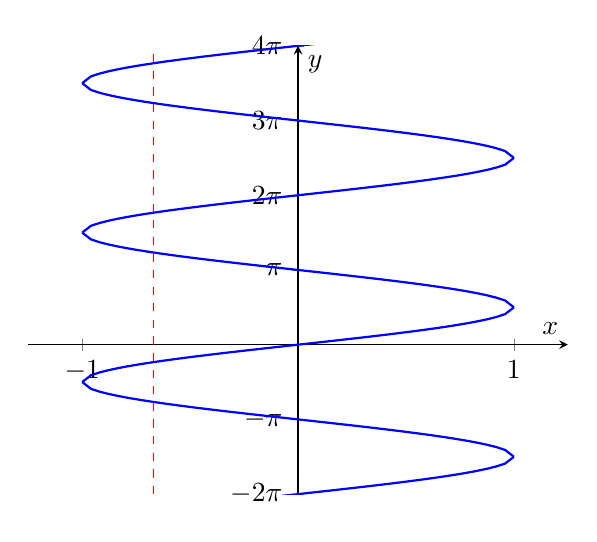
\begin{tikzpicture}
			\begin{axis}
			[axis lines = center, 
			xlabel=$x$,
			ymin=-360,
			ymax=720, 
			ytick={-360, -180, 0, 180, 360, 540, 720}, 
			yticklabels={$-2\pi$, $-\pi$, $0$, 
			$\pi$, $2\pi$, $3\pi$, $4\pi$}, 
			ylabel=$y$,
			xmin = -1.25, 
			xmax=1.25, 
			xtick={-1, 1}]
			\addplot[blue, thick, samples=50, domain=-1:1]{asin(x)};
			\addplot[blue, thick, samples=50, domain=-1:1]{asin(x)-360};
			\addplot[blue, thick, samples=50, domain=-1:1]{-asin(x)-180};
			\addplot[blue, thick, samples=50, domain=-1:1]{-asin(x)+180};
			\addplot[blue, thick, samples=50, domain=-1:1]{asin(x)+360};
			\addplot[blue, thick, samples=50, domain=-1:1]{-asin(x)+540};
			\addplot[blue, thick, samples=50, domain=-1:1]{asin(x)+720};
			\addplot[red, dashed]coordinates{(-0.67, -360) (-0.67, 720)};
			\end{axis}
		\end{tikzpicture}
		\caption{The inverse of an unrestricted $\sin$ function fails the vertical line test}
		\label{fig:arcsinvline}
	\end{figure} 
\end{center}

\section{Restricting the Domain}

The fix, just as with $x^2$ in the inverses chapter, is to use only part of
the sine graph. We keep the piece from $-\frac{\pi}{2}$ to $\frac{\pi}{2}$.
On that piece, sine climbs steadily from $-1$ to $1$, hitting every value
exactly once. So:

\begin{mdframed}[style=important, frametitle={Arcsine}]
$\arcsin x$ is the angle between $-\frac{\pi}{2}$ and $\frac{\pi}{2}$
whose sine is $x$. Its domain is $-1 \le x \le 1$.
\end{mdframed}

\begin{center}
\begin{tikzpicture}
\begin{axis}[axis lines=center, xlabel=$x$, ylabel=$y$,
  xmin=-1.6, xmax=1.8, ymin=-1.8, ymax=1.8,
  xtick={-1,1}, ytick={-1.571,1.571},
  yticklabels={$-\frac{\pi}{2}$,$\frac{\pi}{2}$},
  width=7cm, height=7cm]
\addplot[gray, dashed, domain=-1.571:1.571, samples=60]{sin(deg(x))};
\addplot[sdkblue, thick, domain=-1:1, samples=60]{rad(asin(x))};
\addplot[gray, dotted, domain=-1.6:1.6]{x};
\end{axis}
\end{tikzpicture}

The restricted sine (dashed) and its inverse, $\arcsin x$ (solid). They are
reflections across $y = x$ (dotted).
\end{center}

\index{arccosine}Cosine needs a different piece, because between
$-\frac{\pi}{2}$ and $\frac{\pi}{2}$ cosine goes up and then down. Cosine
falls steadily from 1 to $-1$ between $0$ and $\pi$, so we use that piece.
\index{arctangent}Tangent is steady between $-\frac{\pi}{2}$ and
$\frac{\pi}{2}$, and it takes on every real number there.

\begin{center}
\begin{tabular}{l|l|l}
Function & Input $x$ & Output angle \\
\hline
$\arcsin x$ & $-1 \le x \le 1$ & $-\frac{\pi}{2} \le \theta \le \frac{\pi}{2}$ \\
$\arccos x$ & $-1 \le x \le 1$ & $0 \le \theta \le \pi$ \\
$\arctan x$ & any real number & $-\frac{\pi}{2} < \theta < \frac{\pi}{2}$
\end{tabular}
\end{center}

\textbf{Worked example.} Find $\arcsin\frac{1}{2}$, $\arccos\left(-\frac{1}{2}\right)$,
and $\arctan(-1)$.

\textbf{Solution.}
\begin{itemize}
\item Which angle between $-\frac{\pi}{2}$ and $\frac{\pi}{2}$ has sine
      $\frac{1}{2}$? From the unit circle, $\frac{\pi}{6}$. So
      $\arcsin\frac{1}{2} = \frac{\pi}{6}$.
\item Which angle between $0$ and $\pi$ has cosine $-\frac{1}{2}$? It is
      $\frac{2\pi}{3}$.
\item Which angle between $-\frac{\pi}{2}$ and $\frac{\pi}{2}$ has tangent
      $-1$? It is $-\frac{\pi}{4}$.
\end{itemize}

Watch out for one trap. Since $\sin\frac{5\pi}{6} = \frac{1}{2}$, you might
expect $\arcsin\left(\sin\frac{5\pi}{6}\right) = \frac{5\pi}{6}$. But
arcsin only answers with angles between $-\frac{\pi}{2}$ and
$\frac{\pi}{2}$, so the answer is $\frac{\pi}{6}$.

\begin{Exercise}[title={Exact values}, label=itrig_exact]
Find each value exactly, in radians.
\begin{enumerate}
\item $\arcsin\frac{\sqrt{2}}{2}$
\item $\arccos 0$
\item $\arctan\sqrt{3}$
\item $\arcsin(-1)$
\item $\arccos\left(\cos\left(-\frac{\pi}{3}\right)\right)$
\end{enumerate}
\end{Exercise}
\begin{Answer}[ref=itrig_exact]
\begin{enumerate}
\item $\frac{\pi}{4}$
\item $\frac{\pi}{2}$
\item $\frac{\pi}{3}$
\item $-\frac{\pi}{2}$
\item $\cos\left(-\frac{\pi}{3}\right) = \frac{1}{2}$, and arccos answers
      between $0$ and $\pi$, so the result is $\frac{\pi}{3}$, not
      $-\frac{\pi}{3}$.
\end{enumerate}
\end{Answer}

\section{Finding Angles}

Inverse trig functions shine whenever you know two sides of a right
triangle and want an angle.

\textbf{Worked example.} Back to the ramp. It rises 1 m for every 12 m of
run. What angle does it make with the ground?

\textbf{Solution.} The rise is opposite the angle and the run is adjacent,
so $\tan\theta = \frac{1}{12}$ and
$$\theta = \arctan\frac{1}{12} \approx 0.0831 \text{ radians} \approx 4.76^\circ$$
That is a gentle slope: less than 5 degrees.

On a calculator, the inverse functions are usually above the trig keys,
labeled $\sin^{-1}$, $\cos^{-1}$, and $\tan^{-1}$. Check whether you are in
degrees or radians mode before you trust the answer.

\subsection{Direction of a Vector}

What direction does the vector $[-3, 4]$ point? You might try
$\arctan\frac{4}{-3} \approx -53.1^\circ$. But that points down and to the
right, and $[-3, 4]$ points up and to the left! Arctan only answers between
$-90^\circ$ and $90^\circ$, so it cannot tell $[-3, 4]$ from $[3, -4]$:
both have the same ratio.

Programmers solve this with a two-argument version, \pyfunction{atan2},
which looks at the signs of both components:
\begin{minted}{python}
import math

print(math.degrees(math.atan(4 / -3)))   # -53.13...  (wrong quadrant)
print(math.degrees(math.atan2(4, -3)))   # 126.869...  (correct)
\end{minted}
Notice that \pyfunction{atan2} takes $y$ first, then $x$. Use it whenever
you need the direction of a vector.

\begin{Exercise}[title={Ladder angle}, label=itrig_ladder]
A 6 m ladder leans against a wall with its top 5.5 m above the ground. What
angle does the ladder make with the ground? Safety guides recommend about
$75^\circ$. Is this ladder too steep or too shallow?
\end{Exercise}
\begin{Answer}[ref=itrig_ladder]
The height is opposite the angle and the ladder is the hypotenuse, so
$\theta = \arcsin\frac{5.5}{6} \approx 66.4^\circ$. That is shallower than
$75^\circ$, so the bottom of the ladder is too far from the wall and it
could slide out.
\end{Answer}

\begin{Exercise}[title={A steep road}, label=itrig1]
A road climbs 1.5 m over a horizontal distance of 40 m. What is its angle
of incline, in degrees?
\end{Exercise}
\begin{Answer}[ref=itrig1]
$\theta = \arctan\frac{1.5}{40} \approx 2.15^\circ$.
\end{Answer}
